\section{GPA Embeddings}
This section is devoted to discussing the details of our GPA embeddings.
This will include a thorough discussion of the techniques used to solve the defining equations,
along with a discussion of the coordinates these solutions define.
We find our underlying graphs by orbifolding the graphs in Figures 18b and 21b of \cite{g2_graphs}.
These graphs are shown in Figures~\ref{fig:new-graphs-lvl4} and \ref{fig:new-graphs-lvl3}.

One may give a monoidal functor $F:\GG_2(q_k) \to \GPA(\Gamma)$ by specifying the image of the morphism 
\[
F\left( \skein{skein_figs/trivalent}{0.08} \right) \in \Hom_{\GPA(\Gamma)}(2\to1).
\]
This amounts to giving a list of $M\coloneqq\tr(\Gamma^2\cdot\Gamma)$ complex numbers\footnote{
    We freely switch between using $\Gamma$ to mean the graph itself and the graph's adjacency matrix. }, 
say $a_1,\dots,a_M$. 
Pushing the defining relations of $\GG_2(q_k)$ through $F$, we see that 
these complex numbers satisfy equations in the $a_i$ and $\ol{a_i}$. 
If we assume for now that each $a_i$ is real, then this reduces the system to a collection 
of polynomials in the $a_i$ \footnote{
    This assumption is useful only if it turns out to help us solve the system. 
    In fact, any assumptions we make about this system, if they yield solutions, are in some way valid.
    }.
Once we have the image of the trivalent vertex in hand, we have found an embedding of the planar algebra it generates. 
We can then follow a similar approach to solve for the image
\[
F\left( \skein{skein_figs/Pg}{0.08} \right) \in \Hom_{\GPA(\Gamma)}(2\to2)
\]
to extend the GPA embedding of $\GG_2(q_k)$ to an embedding of $\DD_k$.
Let us discuss our examples.







\subsection{Level 4}
We will begin with level 4.
Let $\Gamma_4$ be the graph given in Figure~\ref{fig:new-graphs-lvl4}.
Set $q_4 \coloneq e^{2\pi i/48}$.
The following result says that we hvae an embedding of $\GG_2(q_4)$ into the GPA on $\Gamma_4$.

\begin{theorem}\label{thm:G2-level3-GPA-emb}
    There is a faithful monoidal functor $F_4:\ol{\GG_2(q_3)} \hookrightarrow \GPA(\Gamma_4)$.
\end{theorem}
\begin{proof}
    See the attached Mathematica notebooks for verification of the necessary equations.
\end{proof}

A proof of the above result amounts to a verification of a system of linear, quadratic, cubic, quartic, and quintiuc equations.
Let 
\[
    (p_1,q_1),\dots,(p_M,q_M)
    \footnote{ See the attached Mathematica files for the specific ordering chosen. }
\]
be the defining basis for $\Hom_{\GPA(\Gamma)}(2\to1)$ ($M=88$ at level 4). Then it must be that 
\[
    F_4 \left( \skein{skein_figs/trivalent}{0.08} \right) = a_1(p_1,q_1)+\cdots+ a_M(p_M,q_M).
\]
The \ref{eq:Bigon} relation, when sent through $F$, becomes the system
\[
    \sum_{i=1}^M a_i(p_i,q_i) \circ \sum_{j=1}^M a_j(q_j,p_j) = k^2 \sum_{e\in E(\Gamma)} (e,e).
\]
This system is quadratic in the $a_i$ since it involves up to two trivalent vertices on either side. 
The \ref{eq:Lolli} and \ref{eq:Rotate} relations therefore determine a system of linear equations; 
the others give cubic, quartic, and quintic equations. 
It is often useful to solve the linear subsystem first and substitute the solution into the quadratic equations. 
For example, when we apply this approach to the \ref{eq:Rotate} equations, we are able to isolate the following resulting equations:

\begin{equation*}
    a_{8}^2+a_{85}^2 = 4-\sqrt{2}+2 \sqrt{3}-\sqrt{6} 
\end{equation*}

\begin{equation*}
    a_{69}^2+\left(1+\sqrt{\frac{3}{2}}\right) a_{8}^2 = \frac{3+\sqrt{3}+\sqrt{6}}{\sqrt{2}} 
\end{equation*}

\begin{equation*}
    a_{69}^2 \left(\left(2+\sqrt{6}\right) a_{8}^2+\left(2+\sqrt{6}\right)
   a_{85}^2-2 \sqrt{2+\sqrt{3}}\right) = 5+\sqrt{2}+\sqrt{3}+2 \sqrt{6}
\end{equation*}

\begin{equation*}
    2 a_{69}^4+\left(5+2 \sqrt{6}\right)
   a_{85}^4 = \left(3+\sqrt{2}+\sqrt{3}+\sqrt{6}\right) a_{85}^2+3
   \sqrt{6}+\sqrt{3}+2 \sqrt{2}+7 
\end{equation*}


Up to three choices of sign, the solution to this system is
\begin{align*}
    a_{8} & = \sqrt{2+\sqrt{3}-\sqrt{2+\sqrt{3}}} \\
    a_{69} & = \sqrt{\frac{1}{2} \left(-1+\sqrt{2}+\sqrt{3}\right)} \\
    a_{85} & = \sqrt{2+\sqrt{3}-\sqrt{2+\sqrt{3}}} \\
\end{align*}
Similar equations containing $a_{31}$, $a_{55}$, and $a_{63}$ appear as well. 
We may repeat this process and obtain the additional values
\begin{align*}
    a_{31} & = \sqrt{2+\sqrt{3}-\sqrt{2+\sqrt{3}}} \\
    a_{55} & = \sqrt{1-\sqrt{\frac{3}{2}}+\frac{1}{\sqrt{2}}} \\
    a_{63} & = \sqrt{2+\sqrt{3}-\sqrt{2+\sqrt{3}}} \\
\end{align*}
These six values begin a cascade of equation solving. 
They, along with the linear solution, reduce many of the original high-order equations to linear. 
We solve those, then repeat the process until we're forced to confront nonlinearity. 
The nonlinearity we encounter forces us to extract square roots, and ending up with a few degree-16 algebraic numbers. 
For instance,
\[
    a_{10} = \frac{1}{2} \left(\sqrt{1+\sqrt{6-3 \sqrt{3}}}+\sqrt{\sqrt{2+\sqrt{3}}-1}\right).
\]

Up to sign, the coordinates of $F_4 \left( \skein{skein_figs/trivalent}{0.08} \right)$ 
take on the following values:
\begin{align*}
    \alpha_1 & = \sqrt{\frac{1}{2} \left(1+2 \sqrt{2}+\sqrt{3}+\sqrt{6}\right)} \\
    \alpha_2 & = \sqrt{\frac{1}{2} \left(-1+\sqrt{2}+\sqrt{3}\right)} \\
    \alpha_3 & = \sqrt{\frac{3}{2} \left(\sqrt{2+\sqrt{3}}-1\right)} \\
    \alpha_4 & = \sqrt{2+\sqrt{3}-\sqrt{2+\sqrt{3}}} \\
    \alpha_5 & = \sqrt{\frac{1}{2} \left(\sqrt{2+\sqrt{3}}-1\right)}  \\
    \alpha_6 & = \sqrt{\frac{1}{2} \left(\sqrt{3}+\sqrt{2+\sqrt{3}}\right)} \\
    \alpha_7 & = \sqrt{1-\sqrt{\frac{3}{2}}+\frac{1}{\sqrt{2}}}  \\
    \alpha_8 & = \frac{1}{2} \left(\sqrt{1+\sqrt{6-3 \sqrt{3}}}-\sqrt{\sqrt{2+\sqrt{3}}-1}\right) \\
    \alpha_9 & = \frac{1}{2} \left(\sqrt{1+\sqrt{6-3 \sqrt{3}}}+\sqrt{\sqrt{2+\sqrt{3}}-1}\right) \\
\end{align*}


\subsection{Extension of level 4}
With our embedding of $\GG_2(q_4)$, i.e. the coordinates of $F_4 \left( \skein{skein_figs/trivalent}{0.08} \right)$, in hand, 
we now know where to find a subcategory of $\GPA(\Gamma_4)$ isomorphic to $\GG_2(q_4)$.
To enlarge this copy of $\GG_2(q_4)$ to a $\Z_n$-like extension, we miust find 
and element of $\Hom_{\GPA(\Gamma_4)}(2\to 2)$ which captures the behavior of 
the idempotent $\skein{skein_figs/Pg}{0.08}$.

To this end, we take a similar approach to the one discusses above.


\begin{theorem}\label{thm:D4-GPA-emg}
    There exists an element $P_4 \in\Hom_{\GPA(\Gamma_4)}(2\to 2)$ satisfying the relations (), (), (), (), and (), 
    with structure constants given by those in Definition~\ref{def:D4}.
\end{theorem}
\begin{proof}
    See the attahed Mathemaica notebooks for verification.
\end{proof}


As an immediate consequence of Theorems~\ref{thm:G2-level3-GPA-emb} and \ref{thm:D4-GPA-emg} we have the following corollary.

\begin{corollary}
    The category $\DD_4$ is a nonzero category which is a $\Z_2$-like extension of $\GG_2(q_4)$.
    Furthermore $\ol{\DD_4}$ is unitary.
\end{corollary}
\begin{proof}
    We deduce $\DD_4$ is nonzero by its embedding into a nonzero subcategory of $\GPA(\Gamma_4)$.
    Unitarity of its semisimple quotient follows from unitarity of $\GPA(\Gamma_4)$.
\end{proof}












\begin{figure}
    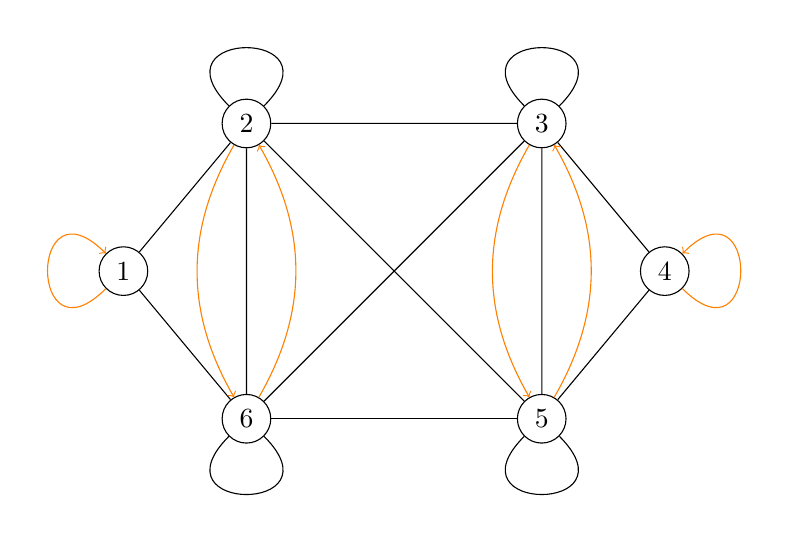
\begin{tikzpicture}[scale=1.25]
        \node[shape=circle,draw=black] (A) at (0,1.5) {1};
        \node[shape=circle,draw=black] (B) at (1.25,3) {2};
        \node[shape=circle,draw=black] (C) at (4.25,3) {3};
        \node[shape=circle,draw=black] (D) at (5.5,1.5) {4};
        \node[shape=circle,draw=black] (E) at (4.25,0) {5};
        \node[shape=circle,draw=black] (F) at (1.25,0) {6};

        % module fusion graph
        \path (B) edge [loop, in=45, out=135, looseness=8] node {} (B);
        \path (C) edge [loop, in=45, out=135, looseness=8] node {} (C);
        \path (E) edge [loop, in=225, out=315, looseness=8] node {} (E);
        \path (F) edge [loop, in=225, out=315, looseness=8] node {} (F);

        \path [-] (A) edge node {} (B);
        \path [-] (A) edge node {} (F);

        \path [-] (B) edge node {} (C);
        \path [-] (B) edge node {} (E);
        \path [-] (B) edge node {} (F);

        \path [-] (C) edge node {} (D);
        \path [-] (C) edge node {} (E);
        \path [-] (C) edge node {} (F);

        \path [-] (D) edge node {} (E);

        \path [-] (E) edge node {} (F);

        % g fusion graph
        \path [->, draw=orange] (A) edge [loop, in=135, out=225, looseness=8] node {} (A);
        \path [->, draw=orange] (D) edge [loop, in=45, out=-45, looseness=8] node {} (D);

        \path [->, draw=orange] (B) edge [bend right] node  {} (F);
        \path [->, draw=orange] (F) edge [bend right] node {} (B);

        \path [->, draw=orange] (C) edge [bend right] node {} (E);
        \path [->, draw=orange] (E) edge [bend right] node {} (C);
    \end{tikzpicture}
    \caption{Fusion graphs at level 4 for $Y$ (black) and $g$ (orange). See \cite[Figure 21b]{g2_graphs}.}
    \label{fig:new-graphs-lvl4}
\end{figure}




\subsection{Level 3}
Let $\Gamma_3$ be the graph given in Figure~\ref{fig:new-graphs-lvl3}.
Set $q_3 \coloneq e^{2\pi i/42}$.
The following result gives us a GPA embedding of $\GG_2(q_3)$.

\begin{theorem}
    There is a faithful monoidal functor $F_3: \ol{\GG_2(q_3)} \to \GPA(\Gamma_3)$.
\end{theorem}
\begin{proof}
    See the attached Mathematica notebooks for verification of the necessary equations.
\end{proof}



\begin{figure}
    \centering
    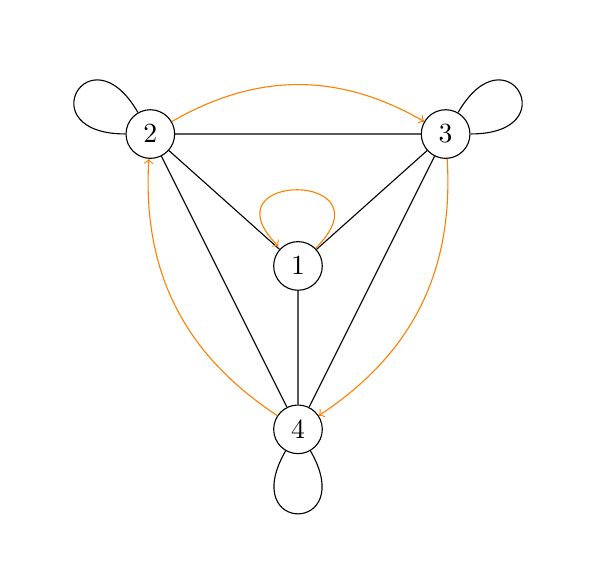
\begin{tikzpicture}[scale=1.25]
        \node[shape=circle,draw=black] (A) at (1.5,1.66) {1};
        \node[shape=circle,draw=black] (B) at (0,3) {2};
        \node[shape=circle,draw=black] (C) at (3,3) {3};
        \node[shape=circle,draw=black] (D) at (1.5,0) {4};
        
        % module fusion graph
        \path (B) edge [loop, in=120, out=180, looseness=10] node {} (B);
        \path (C) edge [loop, in=0, out=60, looseness=10] node {} (C);
        \path (D) edge [loop, in=240, out=300, looseness=10] node {} (D);
        
        \path [-] (D) edge node {} (B);
        \path [-] (B) edge node {} (C);
        \path [-] (C) edge node {} (D);

        \path [-] (A) edge node {} (B);
        \path [-] (A) edge node {} (C);
        \path [-] (A) edge node {} (D);

        % g fusion graph
        \path [->, draw=orange] (B) edge [bend left] node {} (C);
        \path [->, draw=orange] (C) edge [bend left] node {} (D);
        \path [->, draw=orange] (D) edge [bend left] node {} (B);
        \path [->, draw=orange] (A) edge [loop] node {} (A);
    \end{tikzpicture}
    \caption{Fusion graphs at level 3 for $Y$ (black) and $g$ (orange). See \cite[Figure 18b]{g2_graphs}.}
    \label{fig:new-graphs-lvl3}
\end{figure}



\subsection{Extension of level 3}
\begin{theorem}
    There exists an element $P_3  \in\Hom_{\GPA(\Gamma_3)}(2\to 2)$ with the following relations
\end{theorem}

